\section{\gls{bier}: \gls{srt} Analysis}

It is assumed, that the loudness matching (AUTOREF SECTION HERE) is a legit way to provide the same \gls{snr} for both conductors when conducting \gls{bier}.
In order to determine, if under this assumption there is a statistically significant difference in intelligibility between \gls{ac} and \gls{bc}, a paired-sample t-Test is performed.

\begin{table}[H]
\centering
\caption{Average \gls{srt} of the subjects for \gls{ac} and \gls{bc} obtained with \gls{bier}, values are rounded to one digit after the decimal point for representation in the table, not for the underlying calculations.}
\begin{tabular}{lrrrrrrrrrr}
Subject     & 1   & 2    & 3    & 4    & 5    & 6    & 7     & 8     & 9    & 10   \\
Avg. \gls{ac} \gls{srt} & 2.8 & 1.0  & -2.3 & -3.8 & -7.1 & -2.2 & 11.5  & 0.4   & 11.0 & 4.8  \\
Avg. \gls{bc} \gls{srt} & 0.7 & 1.6  & 1.1  & -7.2 & -1.3 & -0.6 & 21.5  & 11.4  & 9.7  & 17.5 \\
\gls{srt}\textsubscript{AC} - \gls{srt}\textsubscript{BC}  & 2.0 & -0.6 & -3.4 & -3.3 & -5.8 & -1.6 & -10.0 & -11.0 & 1.3  & 12.8
\end{tabular}
\end{table}

\begin{figure}[H]
\centering
% This file was created by matlab2tikz.
%
%The latest updates can be retrieved from
%  http://www.mathworks.com/matlabcentral/fileexchange/22022-matlab2tikz-matlab2tikz
%where you can also make suggestions and rate matlab2tikz.
%
\begin{tikzpicture}

\begin{axis}[%
width=120mm, 
height=50mm, 
at={(5mm,5mm)}, 
scale only axis,
xmin=-7.9175,
xmax=22.2175,
xlabel style={font=\color{white!15!black}},
xlabel={Data},
ymin=-1.95996398454005,
ymax=1.95996398454005,
ytick={-3.09023230616781,-2.74778138544499,-2.32634787404084,-2.05374891063182,-1.64485362695147,-1.2815515655446,-0.674489750196082,0,0.674489750196082,1.2815515655446,1.64485362695147,2.05374891063182,2.32634787404084,2.74778138544499,3.09023230616781},
yticklabels={{0.001},{0.003},{0.01},{0.02},{0.05},{0.10},{0.25},{0.50},{0.75},{0.90},{0.95},{0.98},{0.99},{0.997},{0.999}},
ylabel style={font=\color{white!15!black}},
ylabel={Probability},
axis background/.style={fill=white},
title style={font=\bfseries},
title={Normal Probability Plot},
axis x line*=bottom,
axis y line*=left,
xmajorgrids,
ymajorgrids,
legend style={legend cell align=left, align=left, draw=white!15!black}
]


\addplot [color=color1]
  table[row sep=crcr]{%
-2.25	-0.674489750196082\\
4.75	0.674489750196082\\
};
\addlegendentry{\gls{ac}, Gaussian Fit}

\addplot [color=color2, draw=none, mark=+, mark options={solid, blue}]
  table[row sep=crcr]{%
-7.1	-1.64485362695147\\
-3.85	-1.03643338949379\\
-2.25	-0.674489750196082\\
-2.2	-0.385320466407568\\
0.365	-0.125661346855074\\
1.025	0.125661346855074\\
2.75	0.385320466407568\\
4.75	0.674489750196082\\
11	1.03643338949379\\
11.5	1.64485362695147\\
};
\addlegendentry{\gls{ac}, Subject Data}



\addplot [color=color3]
  table[row sep=crcr]{%
-0.603	-0.674489750196082\\
11.35	0.674489750196082\\
};
\addlegendentry{\gls{bc}, Gaussian Fit}

\addplot [color=color4, draw=none, mark=+, mark options={solid, blue}]
  table[row sep=crcr]{%
-7.2	-1.64485362695147\\
-1.285	-1.03643338949379\\
-0.603	-0.674489750196082\\
0.747	-0.385320466407568\\
1.145	-0.125661346855074\\
1.625	0.125661346855074\\
9.7	0.385320466407568\\
11.35	0.674489750196082\\
17.5	1.03643338949379\\
21.5	1.64485362695147\\
};
\addlegendentry{\gls{bc}, Subject Data}
\addplot [color=red, dashdotted]
  table[row sep=crcr]{%
-7.2	-1.41900725744005\\
21.5	1.81998811286491\\
};
%\addlegendentry{data4}
\addplot [color=red, dashdotted]
  table[row sep=crcr]{%
-7.1	-1.60913983261065\\
11.5	1.97529141128853\\
};
%\addlegendentry{data1}

\end{axis}
\end{tikzpicture}%
\caption{Bone Air Thing}
\label{fig:srt_normal}
\end{figure}

\section{\gls{snr} Based Decomposition of the \gls{bier} results}



\begin{figure}[H]
\centering
% This file was created by matlab2tikz.
%
%The latest updates can be retrieved from
%  http://www.mathworks.com/matlabcentral/fileexchange/22022-matlab2tikz-matlab2tikz
%where you can also make suggestions and rate matlab2tikz.
%
\definecolor{mycolor1}{rgb}{0.00000,0.44700,0.74100}%
\definecolor{mycolor2}{rgb}{0.85000,0.32500,0.09800}%
%
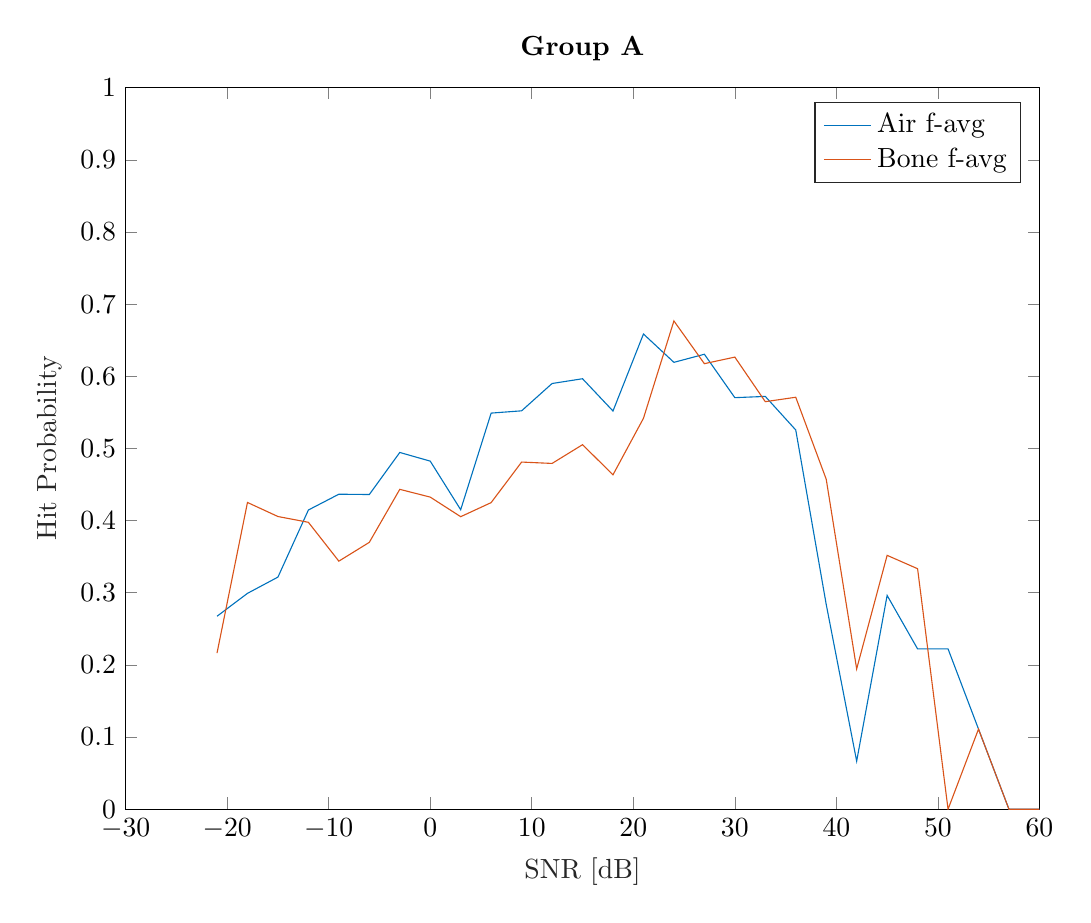
\begin{tikzpicture}

\begin{axis}[%
width=4.569in,
height=3.608in,
at={(0.766in,0.487in)},
scale only axis,
xmin=-30,
xmax=60,
xlabel style={font=\color{white!15!black}},
xlabel={SNR [dB]},
ymin=0,
ymax=1,
ylabel style={font=\color{white!15!black}},
ylabel={Hit Probability},
axis background/.style={fill=white},
title style={font=\bfseries},
title={Group A},
legend style={legend cell align=left, align=left, draw=white!15!black}
]
\addplot [color=mycolor1]
  table[row sep=crcr]{%
-21	0.267436267436267\\
-18	0.299190787426082\\
-15	0.321700902583256\\
-12	0.414691027926322\\
-9	0.436563720554949\\
-6	0.436149190315857\\
-3	0.494428111193677\\
0	0.482417342690147\\
3	0.415080163119379\\
6	0.548985371926549\\
9	0.552129500298837\\
12	0.589983164983165\\
15	0.596593471696671\\
18	0.551860630292003\\
21	0.658608058608059\\
24	0.619312169312169\\
27	0.630537400145243\\
30	0.57037037037037\\
33	0.572089947089947\\
36	0.525599128540305\\
39	0.283950617283951\\
42	0.0666666666666667\\
45	0.296296296296296\\
48	0.222222222222222\\
51	0.222222222222222\\
54	0.111111111111111\\
57	0\\
60	0\\
};
\addlegendentry{Air f-avg}

\addplot [color=mycolor2]
  table[row sep=crcr]{%
-21	0.216402116402116\\
-18	0.425132275132275\\
-15	0.405657451710083\\
-12	0.397647577549538\\
-9	0.343807118807119\\
-6	0.369869890458126\\
-3	0.44331667826979\\
0	0.432574107083911\\
3	0.405417664799816\\
6	0.42493425274732\\
9	0.481119509780168\\
12	0.479222629222629\\
15	0.505197539191572\\
18	0.463492063492064\\
21	0.541757443718228\\
24	0.676708437761069\\
27	0.617460317460317\\
30	0.626577126577126\\
33	0.564814814814815\\
36	0.570940170940171\\
39	0.457407407407407\\
42	0.194444444444444\\
45	0.351851851851852\\
48	0.333333333333333\\
51	0\\
54	0.111111111111111\\
57	0\\
60	0\\
};
\addlegendentry{Bone f-avg}

\end{axis}
\end{tikzpicture}%
\caption{Probability of correct recognition over \gls{snr}, Subject Group A, the x-calibration is questionable}
\label{fig:group_A_decomp}
\end{figure}


\begin{figure}[H]
\centering
% This file was created by matlab2tikz.
%
%The latest updates can be retrieved from
%  http://www.mathworks.com/matlabcentral/fileexchange/22022-matlab2tikz-matlab2tikz
%where you can also make suggestions and rate matlab2tikz.
%
\definecolor{mycolor1}{rgb}{0.00000,0.44700,0.74100}%
\definecolor{mycolor2}{rgb}{0.85000,0.32500,0.09800}%
%
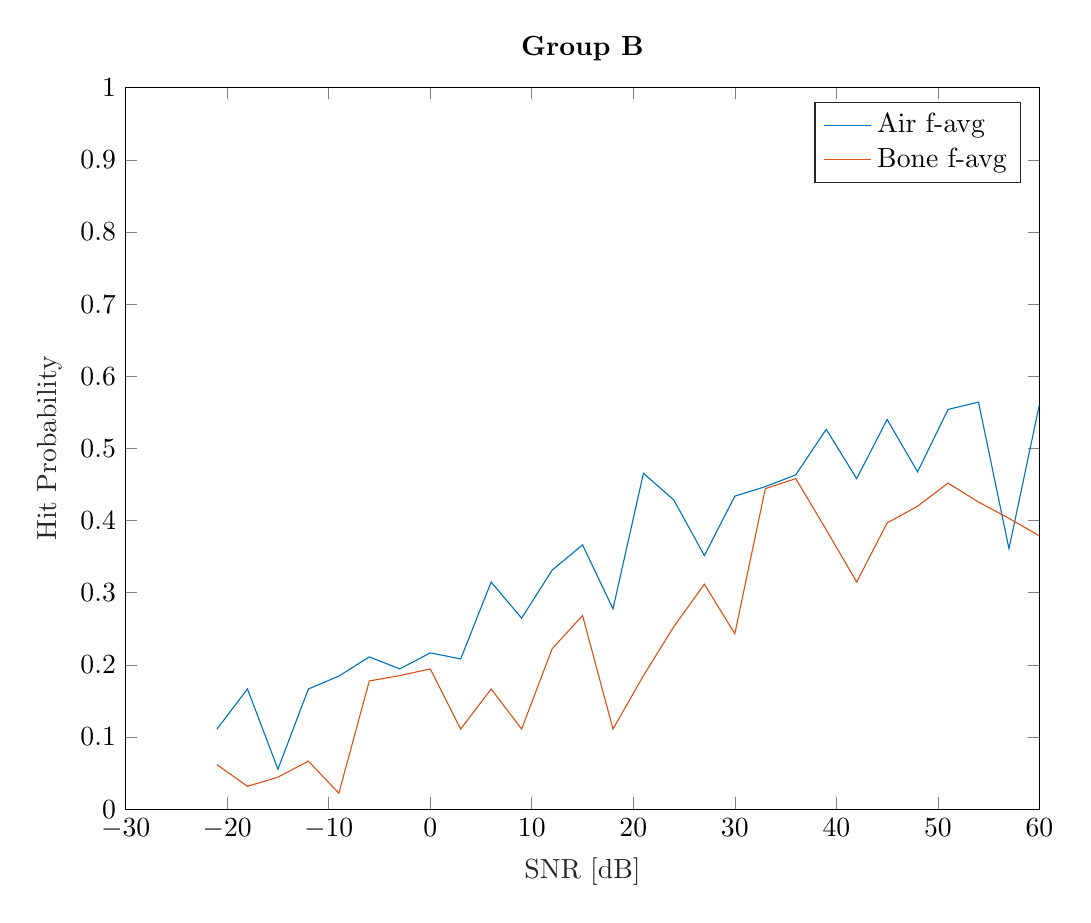
\begin{tikzpicture}

\begin{axis}[%
width=4.569in,
height=3.608in,
at={(0.766in,0.487in)},
scale only axis,
xmin=-30,
xmax=60,
xlabel style={font=\color{white!15!black}},
xlabel={SNR [dB]},
ymin=0,
ymax=1,
ylabel style={font=\color{white!15!black}},
ylabel={Hit Probability},
axis background/.style={fill=white},
title style={font=\bfseries},
title={Group B},
legend style={legend cell align=left, align=left, draw=white!15!black}
]
\addplot [color=mycolor1]
  table[row sep=crcr]{%
-21	0.111111111111111\\
-18	0.166666666666667\\
-15	0.0555555555555556\\
-12	0.166666666666667\\
-9	0.18452380952381\\
-6	0.211111111111111\\
-3	0.194444444444444\\
0	0.216666666666667\\
3	0.208333333333333\\
6	0.314814814814815\\
9	0.264790764790765\\
12	0.331208914542248\\
15	0.366402116402116\\
18	0.277673561006894\\
21	0.465644540644541\\
24	0.428337095003762\\
27	0.351571268237935\\
30	0.433890492223825\\
33	0.447041847041847\\
36	0.463425925925926\\
39	0.526455026455026\\
42	0.458173924840592\\
45	0.540123456790124\\
48	0.467592592592593\\
51	0.554059829059829\\
54	0.564197530864198\\
57	0.361111111111111\\
60	0.560846560846561\\
};
\addlegendentry{Air f-avg}

\addplot [color=mycolor2]
  table[row sep=crcr]{%
-21	0.0617283950617284\\
-18	0.0317460317460317\\
-15	0.0444444444444444\\
-12	0.0666666666666667\\
-9	0.0222222222222222\\
-6	0.177777777777778\\
-3	0.185185185185185\\
0	0.194444444444444\\
3	0.111111111111111\\
6	0.166666666666667\\
9	0.111111111111111\\
12	0.222222222222222\\
15	0.268518518518518\\
18	0.111111111111111\\
21	0.185185185185185\\
24	0.253174603174603\\
27	0.311904761904762\\
30	0.24320987654321\\
33	0.444203944203944\\
36	0.458201058201058\\
39	0.387401795735129\\
42	0.314927048260382\\
45	0.396693121693122\\
48	0.419949494949495\\
51	0.451952060285394\\
54	0.425705467372134\\
57	0.403174603174603\\
60	0.378835978835979\\
};
\addlegendentry{Bone f-avg}

\end{axis}


\end{tikzpicture}%
\caption{Probability of correct recognition over \gls{snr}, Subject Group B, the y-calibration is questionable}
\label{fig:group_B_decomp}
\end{figure}

